%%%%%%%%%%%%%%%%%%%%%%%%%%%%%%%%%%%%%%%%%%%%%%%%%%%%%%%%%%%%%%%%%%%%%%%%%%%%%%%%%%%%%%%%%%%%%%%%
\section{Aplicación de la ecuación de Fisher-Kolmogorov}

En esta sección aplicaremos el método de diferencias finitas desarrollado en la sección \ref{diferenaciasfinitas} para la ecuación \eqref{eq: jisus} de Fisher-Kolmogorov  y estudiaremos el comportamiento de las soluciones para distintos valores de los parámetros de difusión y proliferación.\\

Como ya hemos mencionado, la ecuación de Fisher- Kolmogorov (FK) se utiliza en la modelación de tumores cerebrales (gliomas), describiendo el comportamiento de una densidad $P=P(x,t)$ de células cancerígenas que pueden migrar y proliferar, y la cual viene definida por: 

$$\dfrac{\partial P}{\partial t}=d\dfrac{\partial^{2}P}{\partial x^{2}}+\rho(1-\dfrac{P}{\overline{P}})P,\quad x\in[a,b],\,t\geq 0,$$

donde $d,\,\rho$ y $\overline{P}$ son constantes que representan el coeficiente de difusión (migración) celular, la tasa de proliferación y densidad tisular máxima, respectivamente. Notar que las unidades de $P$ y $\overline{P}$ son número de células/longitud, $d$ se mide en longitud$^{2}$/ tiempo y $\rho$ es inversamente proporcional al tiempo. \\

El intervalo espacial donde se resuelve es $[a,b]$, escogiendo a y b de manera adecuada y recordar que la ecuación de FK se suplementaba normalmente con condiciones de frontera del tipo Neumann.\\

La ecuación de FK se puede simplificar si definimos una nueva variable $u(x,t)=P(x,t)/\overline{P}$, de manera que $0\leq u(x,t)\leq 1$ para todo $x\in[a,b]$ y $t>0$. De esta manera se considera en nuestra \textbf{simulación la EDP normalizada}:

$$u_{_{t}}=du_{_{xx}}+\rho(1-u)u, x\in[a,b],t>0$$

la cual coincide con la estudiada previamente.

\subsection{Problema de aplicación} \label{problemasuelto}
Supongamos que el tumor esta confinada en una region cuya representación es $[-\frac{L}{2},\frac{L}{2}]$, tomando $L=6\,cm$ y se utiliza como la condición inicial la siguiente función:

$$u_{0}=U_{0}\,exp\left(-\dfrac{x^2}{\sigma^2}\right)$$

Lo cual supone que las células cancerígenas se distribuyen en el tejido mediante una distribución del tipo gaussiana y donde la constante(amplitud) $0<U_0<1$ se toma en el rango de valores $U_{_{0}}\in[10^{-3},10^{-1}]$. Los parámetros de difusión y proliferación se supone que cumplen $d\in[1,10^{3}]mm^{2}/$año y $\rho\in[10^{-1},10^{2}]$año$^{-1}$. El intervalo de tiempo que se quiere explorar es $t\in[0,T]$ con $T\in[10^{-1},10]$años.\\

El parámetro restante $\sigma$, se elige de manera que la distribución espacial inicial del tumor esté confinada en una región suficientemente pequeña del intervalo $[-L/2,L/2]$. Para este caso supondremos que $\sigma^2=0\mbox{.}1$\\

Se pretende ver cómo la solución de nuestro problema varía en función de los parámetros $d$ y $\rho$. Para esto fue implementado un código Matlab que nos permitirá resolver el problema de manera eficiente.

\subsection{Código Matlab para la ecuación FK}
\begin{lstlisting}[language=matlab]
	%-----------------------------------------------------------
	%           APLICACION DE LA ECUACION DE FISHER-KOlMOGOROV
	%-----------------------------------------------------------
	%                  Ut = d*Uxx + f(U) % ecuacion de Fisher
	% f(U) : Esta aplicacion describe la tasa de crecimiento 
	% y muerte de las celulas (modelo Logistico). 
	% d    : Constante de difusion.
	%
	function u = FKi(xl,xr,yb,yt,m,n,d,rho)
	
	% ENTRADA : 
	% Posicion  -> [x1,xr], Tiempo    -> [yb,yt]
	% Tamamo de paso en la posicion (x) : h
	% Tamamo de paso en el tiempo (t)   : k
	
	g=@(x) 0.1*exp(-(x.^2)/0.1); % condicion inicial
	h = (xr-xl)/(m-1); % paso espacial 
	k = (yt-yb)/(n-1); % paso temporal
	sigma = d*k/h^2;
	disp('sigma')
	disp(sigma)
	% Inicializamos la matriz solucion y vectores posicion y tiempo
	u=zeros(m,n);
	x=zeros(1,m);
	t=zeros(1,n);
	for j=1:m
	x(j) = xl + (j-1)*h;
	end
	for j=1:n
	t(j) = yb+(j-1)*k;
	end
	% Imponemos la condicion inicial u(x,0)
	for j=1:m
	u(j,1) = g(x(j));
	end
	% Formula de recurrencia explicita
	for j=1:n-1
	for i=2:m-1
	u(i,j+1)=u(i,j)+sigma*(u(i+1,j)-2*u(i,j)+u(i-1,j))+k*rho*(1-u(i,j))*u(i,j);
	end
	u(1,j+1) = u(1,j)+ sigma*(2*u(2,j)-2*u(1,j))+k*rho*(1-u(1,j))*u(1,j);
	u(m,j+1) = u(m,j)+ sigma*(2*u(m-1,j)-2*u(m,j))+k*rho*(1-u(m,j))*u(m,j);
	end
	% Dibujar
	surf(t,x,u)
	% Etiqueta :
	xlabel('t', 'fontname', 'Times new Roman', 'fontsize', 15) % Eje t
	ylabel('x', 'fontname', 'Times new Roman', 'fontsize', 15) % Eje x
	zlabel('u(x,t)', 'fontname', 'Times new Roman', 'fontsize', 15)
	colormap hsv
	colorbar
	end % Final del programa
\end{lstlisting}

\subsection{Solución del Problema mediante FK}
Del problema planteado en \ref{problemasuelto} supongamos los parámetros fijos para los análisis, esto es, $U_0=0\mbox{.}1$, una partición en $m=9$ intervalos de eje espacial, analizaremos para $T= 1$ año, $L=6$, $Sigma^2=0.1$ y la partición $n$ del eje temporal lo suficientemente grande para que el método funcione. Así se llega al siguiente expresión matemática:
\[
\left\{ \begin{array}{lcl}
	\dfrac{\partial u}{\partial t}=d\dfrac{\partial^{2}u}{\partial x^{2}}+\rho(1-u)u     &                      &              \\
	&                      &              \\
	u_{_{x}}(-3,t)=u_{_{x}}(3,t)=0 &                      &     \\
	&                      &              \\
	u(x,0)=0\mbox{.}1\,exp\left(\dfrac{x^{2}}{0.1}\right)                   
\end{array}
\right.
\]
Analizaremos dos casos:
\subsubsection{Es constante el parámetro $\rho$ de proliferación}
Supondremos que $\rho=10$ permanece constante:

\begin{enumerate}
	\item Para $d=1$. Consideramos $n=9$, luego introducimos la siguiente expresión en Matlab $w=\text{FKi}(-3,3,0,1,9,9,1,10)$
				\begin{figure}[H]
					\centering
					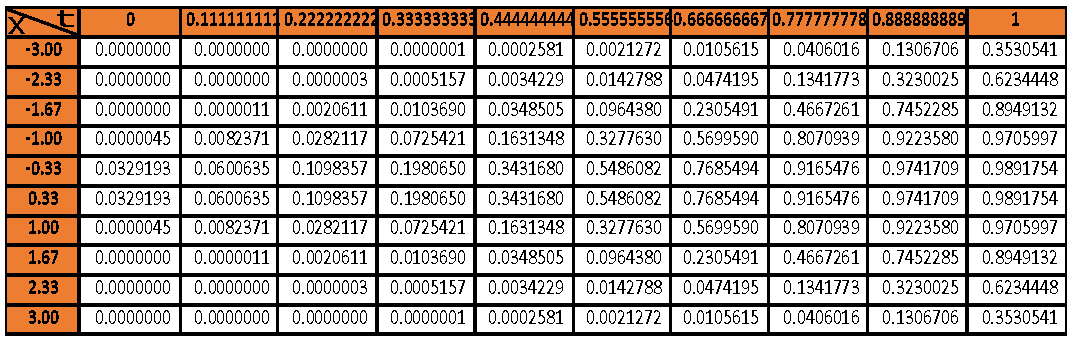
\includegraphics[scale=0.9]{simulacion/tablad1.pdf}
					\caption{{\footnotesize Tabla de iteraciones obtenidas con Matlab para $d=1$ y $\rho =10$}}
				\end{figure}
	\item Para $d=10$. Consideramos $n=99$, luego introducimos la siguiente expresión en Matlab $w=\text{FKi}(-3,3,0,1,9,99,10,10)$
				\begin{figure}[H]
					\centering
					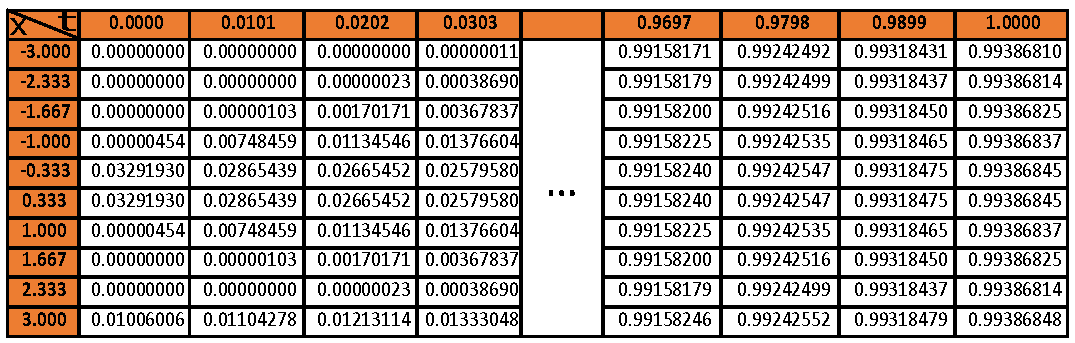
\includegraphics[scale=0.9]{simulacion/tablad10.pdf}
					\caption{{\footnotesize Tabla de iteraciones obtenida con Matlab para $d=10$ y $\rho =10$}}
				\end{figure}
	\item También podemos observar sus gráficas
				\begin{figure}[h]
					\centering
					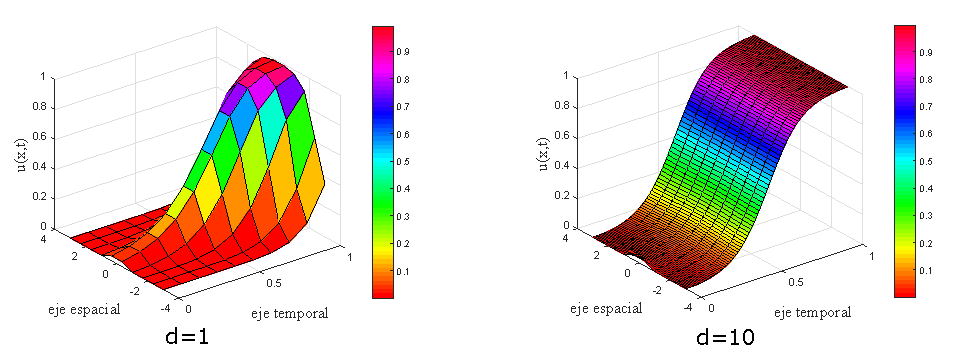
\includegraphics[scale=1]{simulacion/graficodeD.pdf}
					\caption{{\footnotesize Solución para un parámetro de difusión muy pequeña en la izquierda y una difusión grande en la derecha}}
					\label{figuraD}
				\end{figure}
	
\end{enumerate}

\subsubsection{Es constante el coeficiente $d$ de difusión}
Supondremos que $d=10$ permanece constante:

\begin{enumerate}
	\item Para $\rho=0\mbox{.}1$. Consideramos $n=69$, luego introducimos la siguiente expresión en Matlab $w=\text{FKi}(-3,3,0,1,9,69,10,0\mbox{.}1)$
	\begin{figure}[H]
		\centering
		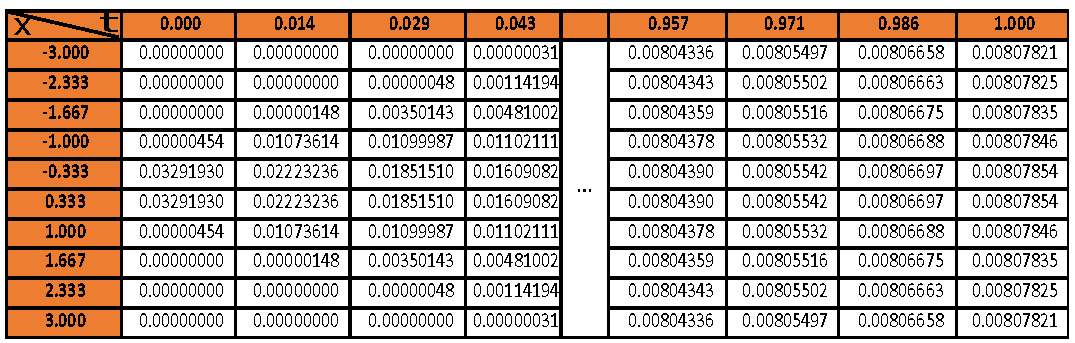
\includegraphics[scale=0.9]{simulacion/tabladrho01.pdf}
		\caption{{\footnotesize Tabla de iteraciones obtenida con Matlab para $d=10$ y $\rho =0\mbox{.}1$}}
	\end{figure}
	\item Pra $\rho=100$. Consideramos $n=99$, luego introducimos la siguiente expresión en Matlab $w=\text{FKi}(-3,3,0,1,9,99,10,100)$
		\begin{figure}[H]
			\centering
			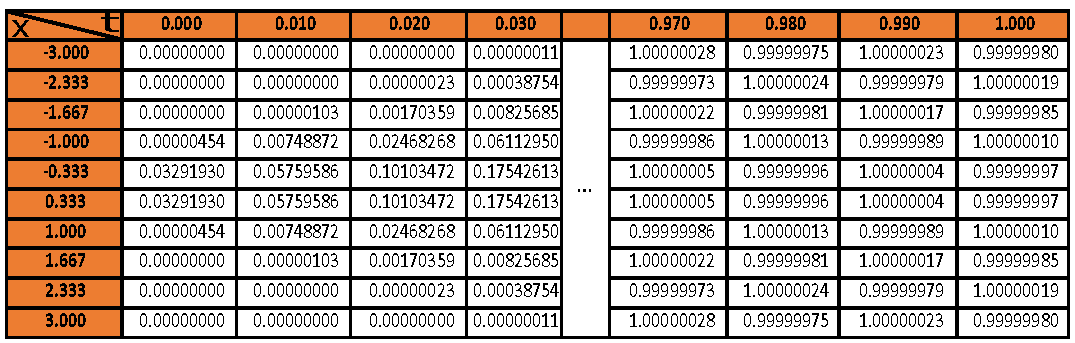
\includegraphics[scale=0.9]{simulacion/tabladrho100.pdf}
			\caption{{\footnotesize Tabla de iteraciones obtenida con Matlab para $d=10$ y $\rho =100$}}
		\end{figure}
	\item También podemos observar sus gráficas 
		\begin{figure}[H]
			\centering
			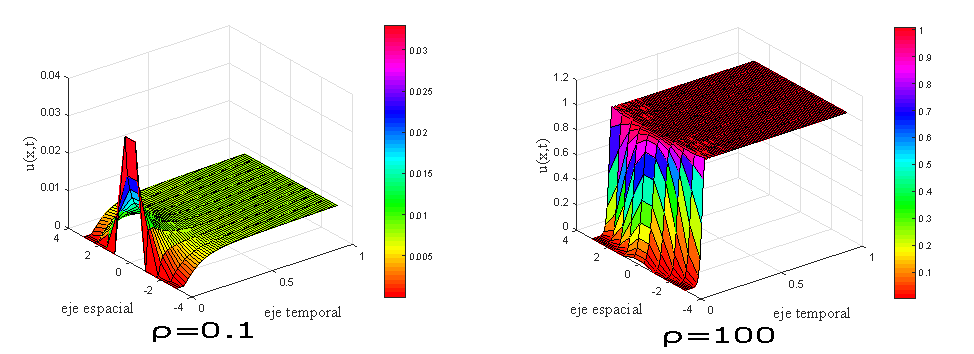
\includegraphics[scale=1]{simulacion/graficoderho.pdf}
			\caption{{\footnotesize Solución para un parámetro de proliferación muy pequeña en la izquierda y una proliferación elevada en la derecha}}
			\label{figuraparaRHO}
		\end{figure}
\end{enumerate}
 

